\documentclass[10pt]{article}
\usepackage{icmlko}

\icmlmeta{IP 파운데이션 월드모델}{299}{제일 잘 가르는 것이 이미 판 안에 있었다}{카테고리가 시장 팝업의 일평균을 네 배 반으로 가르는데 축으로 붙이면 0 이다 --- 채택 검사 셋째를 처음 돌려 이유를 찾았다}

\begin{document}

\twocolumn[
\icmlheader

\begin{abstract}
노트 298 뒤에 하네스 뱅크를 뒤지다 \textbf{카테고리가 제일 센 가름막}인 것을
봤다 --- 앵커 201건에서 크루스칼 $H{=}28.8$($p{=}0.0002$), \texttt{game\_webtoon}
일평균 3,979 대 \texttt{fashion} 810 으로 \textbf{다섯 배}다. 그런데 lab 쪽에서
같은 정보를 축으로 붙인 \texttt{mkt\_cat} 은 노트 285(노트 292가 정정) 에서
$+$0.0048($t{=}0.12$)이었다. \textbf{모순이다} --- 자료에서 제일 잘 가르는 것이
판에 아무것도 안 더한다. 노트 239가 정한 채택 검사 셋 중 \textbf{③ 기존 축과의
겹침}은 이 축에 한 번도 안 돌렸다. 돌렸다. \textbf{① 카테고리는 혼자서 가른다}
--- 시장팝업 학습 101행에서 $H{=}18.4$($p{=}0.0103$), 4,264 대 966 으로 네 배 반.
\textbf{② 그런데 공유 축 둘과 겹친다} --- \texttt{target\_breadth}
($p{=}0.0044$) · \texttt{venue\_prominence}($p{=}0.0134$). \textbf{③ 다섯을
통제하면 안 남는다} --- 능형 잔차에서 $H{=}11.5$, $p{=}\textbf{0.1176}$.
\textbf{카테고리는 이미 판 안에 있었다.} \texttt{target\_breadth} 가
\texttt{ip\_or\_collab} 에서 오는데 그것이 곧 ``IP 를 업었나''이고,
\texttt{game\_webtoon} · \texttt{character} 를 위로 \texttt{fashion} · \texttt{fnb}
를 아래로 놓는 것이 바로 그 축이다. \textbf{그래서 노트 285의 0 이 실패가
아니라 성공의 증거다} --- 판이 이미 그 정보를 갖고 있었다는 뜻이다.
\textbf{"안 오른다"와 "이미 있다"는 다른 말이고, 검사 ③ 이 그것을 가른다.}
\end{abstract}
]

\section{모순을 봤다}

노트 298이 신호 층을 갈라 보는 중에 뱅크의 다른 열들도 같이 쟀다. 제일 센
것이 \textbf{카테고리}였다.

\begin{center}\small
\begin{tabular}{lrr}
\hline
하네스 앵커 201건 & & \\
\hline
카테고리 (크루스칼) & $H{=}28.8$ & $p{=}0.0002$ \\
\texttt{game\_webtoon} 일평균 & 3,979 & \\
\texttt{fashion} 일평균 & 810 & \textbf{다섯 배} \\
\hline
완판 (있음/없음) & $\rho{=}0.085$ & $p{=}0.23$ \\
대기 & $\rho{=}{-}0.014$ & $p{=}0.84$ \\
예약 & $\rho{=}0.013$ & $p{=}0.85$ \\
\hline
\end{tabular}
\end{center}

그런데 lab 에서 같은 정보를 축으로 붙인 \texttt{mkt\_cat} 은 노트 285에서
$+$0.0167 이었고 노트 292가 동률 인공물을 걷어낸 뒤 \textbf{$+$0.0048}
($t{=}0.12$)이다. \textbf{자료에서 제일 잘 가르는 것이 판에 아무것도 안
더한다.}

\paragraph{안 돌린 검사가 있었다} 노트 239 · 285가 정한 채택 검사는 셋이다 ---
① 연도를 통제한 학습 구간 상관 ② 시간 조각 다섯의 부호 일치 ③ \textbf{기존
축과의 겹침}. \texttt{mkt\_cat} 에는 ③ 을 한 번도 안 돌렸다. 그래서
``$+$0.0048 이라 못 쓴다''로만 적혀 있었다.

\section{셋을 돌렸다}

\begin{figure*}[t]
\centering
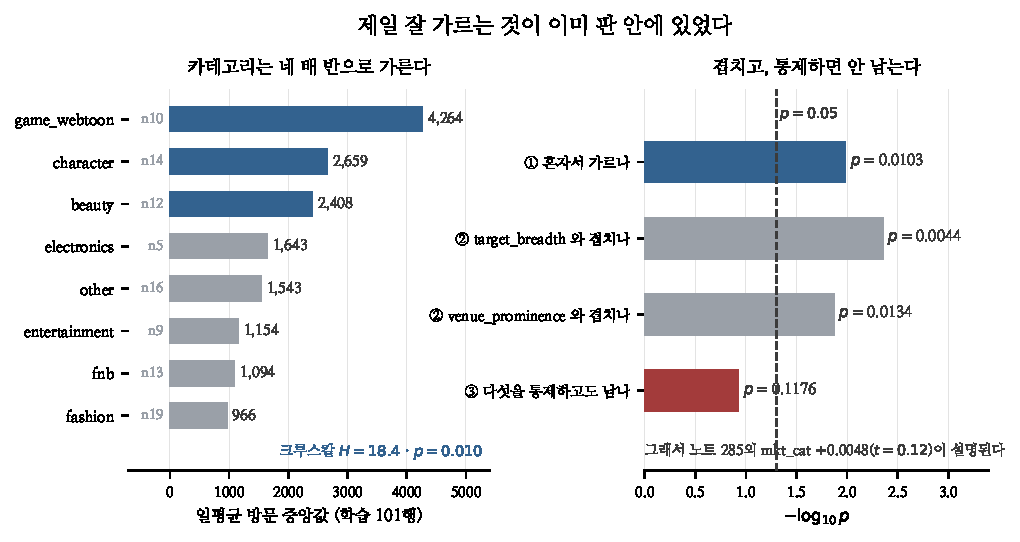
\includegraphics[width=\textwidth]{figs/inside.pdf}
\caption{왼쪽 --- 시장팝업 학습 101행의 카테고리별 일평균 중앙값. 오른쪽 ---
채택 검사 셋.}
\end{figure*}

\paragraph{① 혼자서는 가른다}

\begin{center}\footnotesize
\begin{tabular}{lrr}
\hline
시장팝업 학습 101행 & $n$ & 일평균 중앙 \\
\hline
\texttt{game\_webtoon} & 10 & \textbf{4,264} \\
\texttt{character} & 14 & 2,659 \\
\texttt{beauty} & 12 & 2,408 \\
\texttt{electronics} & 5 & 1,643 \\
\texttt{other} & 16 & 1,543 \\
\texttt{entertainment} & 9 & 1,154 \\
\texttt{fnb} & 13 & 1,094 \\
\texttt{fashion} & 19 & \textbf{966} \\
\hline
\multicolumn{3}{l}{크루스칼 $H{=}18.4$ · $p{=}0.0103$ · \textbf{네 배 반}} \\
\hline
\end{tabular}
\end{center}

\paragraph{② 그런데 공유 축과 겹친다}

\begin{center}\footnotesize
\begin{tabular}{lrrl}
\hline
축 & 관측 & $H$ & $p$ \\
\hline
\texttt{target\_breadth} & 101 & 20.6 & \textbf{0.0044} \\
\texttt{venue\_prominence} & 101 & 17.7 & \textbf{0.0134} \\
\texttt{goods\_scale} & 93 & 12.4 & 0.0884 \\
\texttt{entry\_friction} & 72 & 9.1 & 0.1036 \\
\texttt{media\_push} & 0 & --- & 마스크 0 \\
\hline
\end{tabular}
\end{center}

\paragraph{③ 통제하면 안 남는다} 공유 축 다섯(값 $+$ 관측 표시자 열 개)으로
능형을 적합하고($R^2{=}0.166$) 그 \textbf{잔차}에 카테고리를 다시 물었다.

\begin{center}\small
\begin{tabular}{lrr}
\hline
& $H$ & $p$ \\
\hline
카테고리 (통제 전) & 18.4 & 0.0103 \\
카테고리 (통제 후) & 11.5 & \textbf{0.1176} \\
\hline
\end{tabular}
\end{center}

\textbf{남지 않는다.}

\section{어느 축이 그 일을 하고 있나}

\texttt{target\_breadth} 는 \texttt{ip\_or\_collab} 에서 온다(\texttt{ingest/
market\_axes.py}) --- ``IP 나 협업을 업었나''다. 그리고 카테고리 순서가 정확히
그 무늬다: \texttt{game\_webtoon} · \texttt{character} 가 위, \texttt{fashion} ·
\texttt{fnb} 가 아래다. \textbf{카테고리 이름이 하는 일을 IP 여부가 이미 하고
있다.}

\texttt{venue\_prominence}(\texttt{ip\_history.prior\_count})도 같은 방향이다 ---
반복 개최되는 IP 팝업이 게임·캐릭터 쪽에 몰린다.

\section{그래서 0 의 뜻이 바뀐다}

\begin{center}\footnotesize
\begin{tabular}{ll}
\hline
0 의 두 가지 뜻 & 가르는 법 \\
\hline
\textbf{안 오른다} --- 정보가 없다 & ① 이 떨어진다 \\
\textbf{이미 있다} --- 판이 갖고 있다 & ① 통과 · ③ 떨어진다 \\
\hline
\end{tabular}
\end{center}

\texttt{mkt\_cat} 은 \textbf{둘째}다. 검사 ① 을 통과하고(혼자서 $p{=}0.010$)
검사 ③ 에서 떨어진다($p{=}0.118$). \textbf{$+$0.0048 은 축이 쓸모없다는
뜻이 아니라 판이 이미 그 일을 하고 있다는 뜻이다.}

이것이 실무적으로 다르다 --- 첫째면 \emph{더 좋은 자료를 구하라}이고, 둘째면
\emph{이 자리는 이미 채워졌으니 다른 데를 보라}다. 오늘 여러 번 ``문턱 아래''로
끝냈는데(노트 294 · 296 · 297) \textbf{그중 어느 것이 둘째인지 안 갈랐다.}

\paragraph{남은 것}
\begin{center}\small
\begin{tabular}{ll}
\hline
갈래 & 왜 \\
\hline
검사 ③ 을 나머지에 & 회사 축 · \texttt{pop\_*} 넷 \\
위약 팔 & 신호가 내용이냐 모양이냐 \\
검사 ③ 을 가드로 & ``이미 있음''을 자동으로 적게 \\
\hline
\end{tabular}
\end{center}

\paragraph{규약} \textbf{0 을 보면 검사 ③ 을 돌려 어느 0 인지 갈라라.} 노트
239가 검사 셋을 정해 놓고도 ③ 을 거의 안 돌렸다 --- ① 이 떨어지면 거기서
끝났고 ① 이 통과하면 유보 수를 봤기 때문이다. \textbf{③ 은 유보를 보기 전에
돌아야 하는 검사다.} 그리고 \textbf{제일 세 보이는 열을 의심하라} --- 카테고리는
자료에서 제일 크게 가르는 열이었고, 그래서 \emph{이미 다른 이름으로 판에
들어와 있었다.}

\end{document}
